% \newpage
% \section{\textbf{ CHƯƠNG 4: THIẾT KẾ CƠ SỞ DỮ LIỆU}}

% \textbf{1. posts}

% \begin{table}[H]
% \centering
% \renewcommand{\arraystretch}{1.3}
% \begin{tabular}{|p{4cm}|p{4cm}|p{2cm}|p{2cm}|p{2cm}|}
% \hline
% \textbf{Name} & \textbf{Data Type} & \textbf{Array} & \textbf{Key} & \textbf{Required} \\
% \hline
% \_id         & objectId &  & Yes & Yes \\
% postedBy     & objectId &  &     & Yes \\
% text         & string   &  &     & Yes \\
% text\_vector & double   & Yes &     & Yes \\
% img          & string   &  &     & Yes \\
% likes        & objectId & Yes &     & Yes \\
% likesCount   & double   &  &     & Yes \\
% replies      & string   & Yes &     & Yes \\
% createdAt    & date     &  &     & Yes \\
% updatedAt    & date     &  &     & Yes \\
% \hline
% \end{tabular}
% \caption{Cấu trúc của bảng \texttt{posts}}
% \end{table}


% \textbf{2. chatmessages}

% \begin{table}[H]
% \centering
% \renewcommand{\arraystretch}{1.3}
% \begin{tabular}{|p{4cm}|p{4cm}|p{2cm}|p{2cm}|p{2cm}|}
% \hline
% \textbf{Name} & \textbf{Data Type} & \textbf{Array} & \textbf{Key} & \textbf{Required} \\
% \hline
% \_id         & objectId &  & Yes & Yes \\
% userId       & objectId &  &     & Yes \\
% isUser       & bool     &  &     & Yes \\
% message      & string   &  &     & Yes \\
% createdAt    & date     &  &     & Yes \\
% updatedAt    & date     &  &     & Yes \\
% \hline
% \end{tabular}
% \caption{Cấu trúc của bảng \texttt{chatmessages}}
% \end{table}

% \newpage
% \textbf{3. threads}


% \begin{table}[H]
% \centering
% \renewcommand{\arraystretch}{1.3}
% \begin{tabular}{|p{4cm}|p{4cm}|p{2cm}|p{2cm}|p{2cm}|}
% \hline
% \textbf{Name} & \textbf{Data Type} & \textbf{Array} & \textbf{Key} & \textbf{Required} \\
% \hline
% \_id         & objectId &  & Yes & Yes \\
% userId       & objectId &  &     & Yes \\
% createdAt    & date     &  &     & Yes \\
% lastUsed     & date     &  &     & Yes \\
% threadId     & string   &  &     & Yes \\
% \hline
% \end{tabular}
% \caption{Cấu trúc của bảng \texttt{threads}}
% \end{table}

% \newpage
% \textbf{4. reports}

% \begin{table}[H]
% \centering
% \renewcommand{\arraystretch}{1.3}
% \begin{tabular}{|p{4cm}|p{4cm}|p{2cm}|p{2cm}|p{2cm}|}
% \hline
% \textbf{Name} & \textbf{Data Type} & \textbf{Array} & \textbf{Key} & \textbf{Required} \\
% \hline
% \_id               & objectId &  & Yes & Yes \\
% reportedBy         & any      &  &     & Yes \\
% reportedContent    & objectId &  &     & Yes \\
% contentType        & string   &  &     & Yes \\
% reason             & string   &  &     & Yes \\
% details            & string   &  &     & Yes \\
% status             & string   &  &     & Yes \\
% createdAt          & date     &  &     & Yes \\
% updatedAt          & date     &  &     & Yes \\
% resolvedBy         & objectId &  &     & Yes \\
% postId             & objectId &  &     & Yes \\
% postContent        & string   &  &     & Yes \\
% moderationResult   & string   &  &     & Yes \\
% resolution         & string   &  &     & Yes \\
% severity           & string   &  &     & Yes \\
% reportedByUsername & string   &  &     & Yes \\
% postImage          & any      &  &     & Yes \\
% \hline
% \end{tabular}
% \caption{Cấu trúc của bảng \texttt{reports}}
% \end{table}


% \newpage
% \textbf{5. verifications}

% \begin{table}[H]
% \centering
% \renewcommand{\arraystretch}{1.3}
% \begin{tabular}{|p{4cm}|p{4cm}|p{2cm}|p{2cm}|p{2cm}|}
% \hline
% \textbf{Name} & \textbf{Data Type} & \textbf{Array} & \textbf{Key} & \textbf{Required} \\
% \hline
% \_id         & objectId &  & Yes & Yes \\
% userId       & objectId &  &     & Yes \\
% email        & string   &  &     & Yes \\
% code         & string   &  &     & Yes \\
% createdAt    & date     &  &     & Yes \\
% \hline
% \end{tabular}
% \caption{Cấu trúc của bảng \texttt{verifications}}
% \end{table}

% \newpage
% \textbf{6. messages}

% \begin{table}[H]
% \centering
% \renewcommand{\arraystretch}{1.3}
% \begin{tabular}{|p{4cm}|p{4cm}|p{2cm}|p{2cm}|p{2cm}|}
% \hline
% \textbf{Name} & \textbf{Data Type} & \textbf{Array} & \textbf{Key} & \textbf{Required} \\
% \hline
% \_id          & objectId &  & Yes & Yes \\
% sender        & objectId &  &     & Yes \\
% recipient     & objectId &  &     & Yes \\
% messageType   & string   &  &     & Yes \\
% text          & string   &  &     & Yes \\
% media         & null     &  &     &     \\
% file          & string   &  &     &     \\
% fileName      & null     &  &     &     \\
% fileSize      & null     &  &     &     \\
% fileType      & null     &  &     &     \\
% thumbnailUrl  & null     &  &     &     \\
% duration      & null     &  &     &     \\
% read          & bool     &  &     & Yes \\
% createdAt     & date     &  &     & Yes \\
% updatedAt     & date     &  &     & Yes \\
% cloudinary    & string   &  &     & Yes \\
% fileInfo      & string   &  &     & Yes \\
% mediaDetails  & string   &  &     & Yes \\
% status        & string   &  &     & Yes \\
% img           & string   &  &     & Yes \\
% pending       & bool     &  &     & Yes \\
% \hline
% \end{tabular}
% \caption{Cấu trúc của bảng \texttt{messages}}
% \end{table}
% \newpage
% \textbf{7. users}

% \begin{table}[H]
% \centering
% \renewcommand{\arraystretch}{1.3}
% \begin{tabular}{|p{4cm}|p{4cm}|p{2cm}|p{2cm}|p{2cm}|}
% \hline
% \textbf{Name} & \textbf{Data Type} & \textbf{Array} & \textbf{Key} & \textbf{Required} \\
% \hline
% \_id             & objectId &     & Yes & Yes \\
% name            & string   &     &     & Yes \\
% username        & string   &     &     & Yes \\
% email           & string   &     &     & Yes \\
% password        & string   &     &     & Yes \\
% profilePic      & string   &     &     & Yes \\
% followers       & string   & Yes &     & Yes \\
% following       & string   & Yes &     & Yes \\
% bio             & string   &     &     & Yes \\
% isFrozen        & bool     &     &     & Yes \\
% createdAt       & date     &     &     & Yes \\
% updatedAt       & date     &     &     & Yes \\
% isEmailVerified & any      &     &     & Yes \\
% viewedPosts     & objectId & Yes &     & Yes \\
% lastActive      & date     &     &     & Yes \\
% totalSessionTime & double   &     &     & Yes \\
% likes           & objectId & Yes &     & Yes \\
% isAdmin         & bool     &     &     & Yes \\
% \hline
% \end{tabular}
% \caption{Cấu trúc của bảng \texttt{users}}
% \end{table}
% \newpage
% \textbf{8. notifications}

% \begin{table}[H]
% \centering
% \renewcommand{\arraystretch}{1.3}
% \begin{tabular}{|p{4cm}|p{4cm}|p{2cm}|p{2cm}|p{2cm}|}
% \hline
% \textbf{Name} & \textbf{Data Type} & \textbf{Array} & \textbf{Key} & \textbf{Required} \\
% \hline
% \_id         & objectId &  & Yes & Yes \\
% recipient    & objectId &  &     & Yes \\
% sender       & objectId &  &     & Yes \\
% type         & string   &  &     & Yes \\
% post         & objectId &  &     & Yes \\
% read         & bool     &  &     & Yes \\
% createdAt    & date     &  &     & Yes \\
% updatedAt    & date     &  &     & Yes \\
% \hline
% \end{tabular}
% \caption{Cấu trúc của bảng \texttt{notifications}}
% \end{table}

% \textbf{9. Quan hệ giữa các bảng}

% \begin{itemize}
% \item 1 User có thể tạo nhiều Posts (qua trường postedBy)
% \item 1 User có thể thích nhiều Posts (qua mảng likes)
% \item 1 User có thể xem nhiều Posts (qua mảng viewedPosts)
% \item 1 User có thể gửi nhiều Messages (qua trường sender)
% \item 1 User có thể nhận nhiều Messages (qua trường recipient)
% \item 1 User có thể nhận nhiều Notifications (qua trường recipient)
% \item 1 User có thể tạo nhiều Notifications (qua trường sender)
% \item 1 User có thể có nhiều Chatmessages (qua trường userId)
% \item 1 User có thể có nhiều Threads (qua trường userId)
% \item 1 Post có thể tạo nhiều Notifications (qua trường post)
% \item 1 Post có thể có nhiều Reports (qua trường postId)
% \item 1 User có thể tạo nhiều Reports (qua trường reportedBy)
% \item 1 User có thể xử lý nhiều Reports (qua trường resolvedBy)
% \item 1 Post có thể có nhiều Replies (qua mảng replies)
% \item 1 User có thể theo dõi nhiều Users khác (qua mảng following)
% \item 1 User có thể được nhiều Users khác theo dõi (qua mảng followers)
% \item 1 User có thể có nhiều Verifications (qua trường userId)
% \end{itemize}
% Từ đó xây dựng biểu đồ cơ sở dữ liệu như hình vẽ dưới:

% \begin{figure}[H]
%     \centering
%     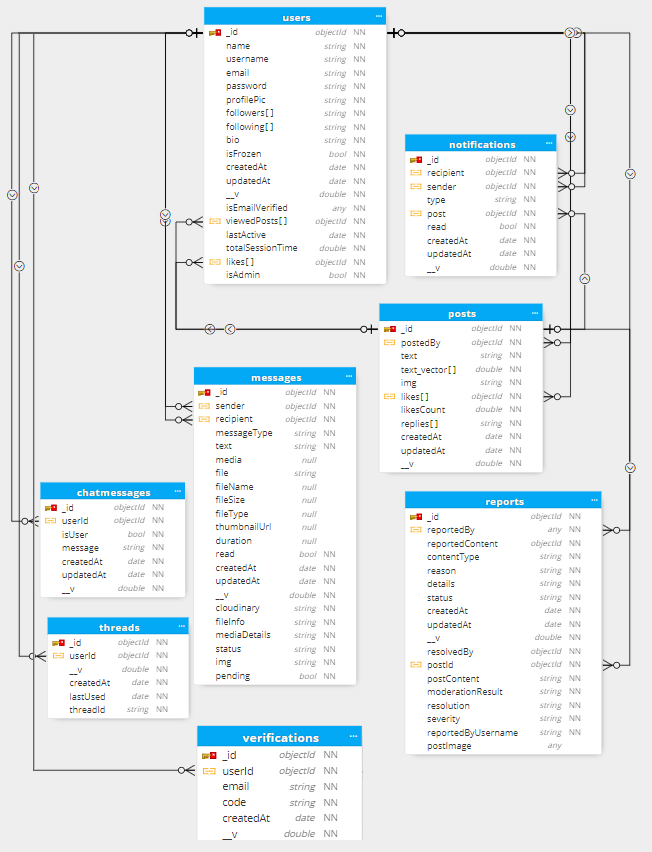
\includegraphics[width=1\textwidth]{image/MoHinh/13.png}
%     \caption{Hình ảnh Quan hệ giữa các bảng}
%     \label{fig:quan_he_giua_cac_banng}
% \end{figure}